\section{NVM}
\subsection{Ram Block}
\subsubsection{Permanent and non-permanent RAM Blocks}
RAM block 可以是永久性的,也可以是非永久性的。永久 RAM 块是只能由一个应用程序访问的 NV 块。 RAM 块的地址是固定的,并存储在 NVM 的配置中。

也可以让多个应用程序访问同一个 NV 块。每个应用程序都使用自己的 RAM 块。在这种情况下,RAM 块称为非永久性的。
由于 RAM 地址未存储在 NVM 配置中(并且可能会变化),因此必须提供一个指针来读取和写入非永久性块。这也是 \lstinline{NVM_WriteALL} 和 \lstinline{NVM_ReadAll} 使用第二个参数传递
非永久 RAM block 地址的原因。

\begin{remark}
异步 API 函数可以由不同的任务重入。因此,多个任务可能同时将 Block 入队,例如写入 job(具有较高优先级的任务可能会中断较低的任务)。
但是不可能将同一个块多次入队(既不能是由不同的任务也不能是由不同的 job)。
因此,例如,如果块 5 的读取作业已排队,则该块的擦除 job 不能在读取 job 完成之前排队。
如果一个块被多个任务使用,这是非永久性 RAM 块的常见任务,应用程序负责同步。当然,例如,如果正在处理擦除请求,则可以读取或写入 RAM 块,而不会对擦除作业的结果产生任何影响。
唯一的问题是 NVM 不向应用程序提供任何信息,即当前正在为块处理什么服务。启动服务的应用程序当然知道,但也使用该块的不同应用程序不知道。
因此,只要块处于挂起状态,这时访问最安全的方法是不要使用 RAM 块。这样可以彻底避免 RAM 不一致。
\end{remark}

\begin{definition}[\lstinline{NvMBlockUseSyncMechanism}]
此参数定义是否为此块使用具有 RAM 镜像和回调例程的显式同步机制,用于将数据传输到 NvM 模块的 RAM 镜像和从 NvM 模块的 RAM 镜像传输数据。
如果使用, \lstinline{NvMReadRamBlockFromNvCallback} 和 \lstinline{NvMWriteRamBlockToNvCallback} 都必须设置为适当函数的名称。
\end{definition}
\begin{definition}[\lstinline{NvMWriteRamBlockToNvCallback}]
  该参数定义了块特定的回调例程,为了让应用程序将数据从 RAM 块复制到 NvM RAM块的镜像,应调用该回调例程。
\end{definition}

\begin{definition}[\lstinline{NvMReadRamBlockFromNvCallback}]
  该参数定义了块特定的回调例程,为了让应用程序将数据从 NvM 模块的镜像复制到 RAM 块,应调用该回调例程。
\end{definition}

NVM 模块支持在应用程序和 NVM间的显式同步机制。实现方式为在 NVM 模块中添加一个 RAM 镜像块。数据在应用程序和NVM模块间通过回调函数进行双向传递,这些回调函数由 NVM模块调用。

每个 Block块可以支持独立配置同步机制。如果配置了同步机制,NVM 模块使用内部 buffer 用作 RAM 块镜像。同样,该块也用于 CRC 计算。buffer 的大小为最大配置 Block 大小加上 CRC 大小。\textbf{实际上大小设置为 256}。如下:

\begin{lstlisting}[language=C,style=C]
  // internal buffer size 
#define NVM_INTERNAL_BUFFER_LENGTH            256uL

// create the internal buffer of size NVM_INTERNAL_BUFFER_LENGTH
VAR(uint8, NVM_PRIVATE_DATA) NvM_InternalBuffer_au8[NVM_INTERNAL_BUFFER_LENGTH];
\end{lstlisting}

为使用同步机制的块配置永久 RAM 块是没有用的。在这种情况下,RAM 块将被忽略。也不建议为使用同步机制的块配置 Init 回调。

\begin{remark}
  如果为块配置了显式同步,则客户端可以在块挂起时修改各自的 RAM 内容(对 NVM 不可见)。在这种情况下,当挂起的读取完成时,请注意它们的值可能会被覆盖。
\end{remark}

\subsubsection{Explicit synchronization mechanism during write requests}
在应用程序发出 \lstinline{NvM_WriteBlock} 后,应用程序可能会修改 RAM 块,直到 NvM 调用回调 \lstinline{NvMWriteRamBlockToNvM} 。
如果调用 \lstinline{NvMWriteRamBlockToNvM} ,应用程序必须向内部 RAM 镜像提供 RAM 块的一致副本。

\subsubsection{Explicit synchronization mechanism during read requests} 
在应用程序发出 \lstinline{NvM_ReadBlock} 后,应用程序可能会修改 RAM 块,直到 NvM 调用例程 \lstinline{NvMReadRamBlockFromNvM} 。
如果调用 \lstinline{NvMReadRamBlockFromNvM} ,则应用程序必须将数据从内部 RAM 镜像复制到 RAM 块。

\subsection{Rom Block}

Rom Block的值由应用程序提供,同样,可以通过初始化回调函数用于提供 Rom 默认值。这些通过配置实现。当然,只可以选择 Rom Block 和 初始化回调函数的其中一种。

Rom 默认值可以通过显式接口调用 \lstinline{NvM_RestoreBlockDefaults()}。在读请求时,也可以隐式的读取默认值。
如以下场景:当从 NVM 存储中没有读取到有效数据,比如由于 CRC 错误或由于底层模块 \lstinline{MEMIF} 报出错误时。

在 block 读操作时,重载了 Rom 默认值,则 block 结果为 \lstinline{NVM_REQ_RESTORED_FROM_ROM}。
直接调用 \lstinline{NvM_RestoreBlockDefaults()} 并不会给出 \lstinline{NVM_REQ_RESTORED_FROM_ROM} 的结果。

\begin{remark}
  上面所说的结果可以通过以下接口获取:
  \begin{lstlisting}[language=C,style=C]
  Std_ReturnType NvM_GetErrorStatus ( NvM_BlockIdType BlockId,  NvM_RequestResultType* RequestResultPtr)
  \end{lstlisting}
\end{remark}

\subsection{The configuration ID}

block 1 NvMConfigBlock是一个特殊的 NV 块,其保存了一个常量\lstinline{NvM_CompiledConfigId_t},该常量和配置项\lstinline{/MICROSAR/NvM/NvMCommon/NvMCompiledConfigId}对应。当\lstinline{ReadAll}时,该Block的值和常量值进行比较,当两个值匹配时,所有的NV
block可认为是有效的,NVM尝试从NV中读取数据。如果值不匹配或者没有读取到有效的configuration ID,则NVM的系统行为如下:

\begin{itemize}
	\item
  当配置项\lstinline{/MICROSAR/NvM/NvMCommon/NvMDynamicConfiguration}为 off 时,不匹配将被忽略,NVM将从NV中尝试读取数据。(normal runtime preparation)。
	\item
  当配置项为on时,所有配置了\lstinline{/MICROSAR/NvM/NvMBlockDescriptor/NvMResistantToChangedSw}的block,将视为 normal runtime preparation,将从NV中尝试读取数据。其他未配置的block将视为 extended runtime preparation。不会从NV中读取数据。
	\item
  所有视为 extended runtime preparation 的block,将被认为是无效的或空的block。因此,配置为 write once 的block将被重写。如果配置了 rom block 或初始化回调函数,则会进行值的初始化。
\end{itemize}

\subsection{Block状态查询}

\subsubsection{\lstinline{NvM_QryBlockRelevantForWriteAll}}

block在满足以下条件后,writeall 阶段可写入NV Block。

\begin{itemize}
\item
  block勾选了 \lstinline{Write all}

  \begin{itemize}
  \item
    使能
    \lstinline{NVM_SET_RAM_BLOCK_STATUS_API}时,当block状态为\lstinline{NVM_STATE_CHANGED_SET}和\lstinline{NVM_STATE_VALID_SET}时,需要写入,否则无需写入。
  \item
    未使能 \lstinline{NVM_SET_RAM_BLOCK_STATUS_API}时,需要写入。
  \end{itemize}
  
\item
  未勾选 \lstinline{Write all},无需写入。
\end{itemize}

\subsubsection{\lstinline{NvM_ApiFlags}}

\begin{figure}
\centering
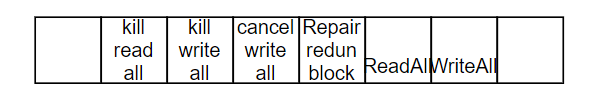
\includegraphics{./pic/NvM_ApiFlags.png}
\caption{nvm-01}
\end{figure}


\subsubsection{readall 和 writeall顺序}

\begin{itemize}
\item
  Write all从block id最大值的到0
\item
  Read all 从0到 id最大值
\end{itemize}

\subsection{CRC机制}

\subsubsection{NvMCalcRamBlockCrc}
% 全局ram block的CRC是否需要计算或重新计算。在\lstinline{Read all}阶段,NVM内部存储读到的CRC值,并进行数据校验和比较。
\begin{remark}
  目前的理解是,NVM 模块通过内部的 CRC buffer 存储 block 的 CRC 值,并在 \lstinline{NVM_ReadAll} 阶段,验证 Ram block 的 CRC值是否一致,一致时避免从NV 中读数据。
\end{remark}

NvMCalcRamBlockCrc 配置影响下的处理流程,如下图所示:

\begin{figure}[ht]
  \centering
  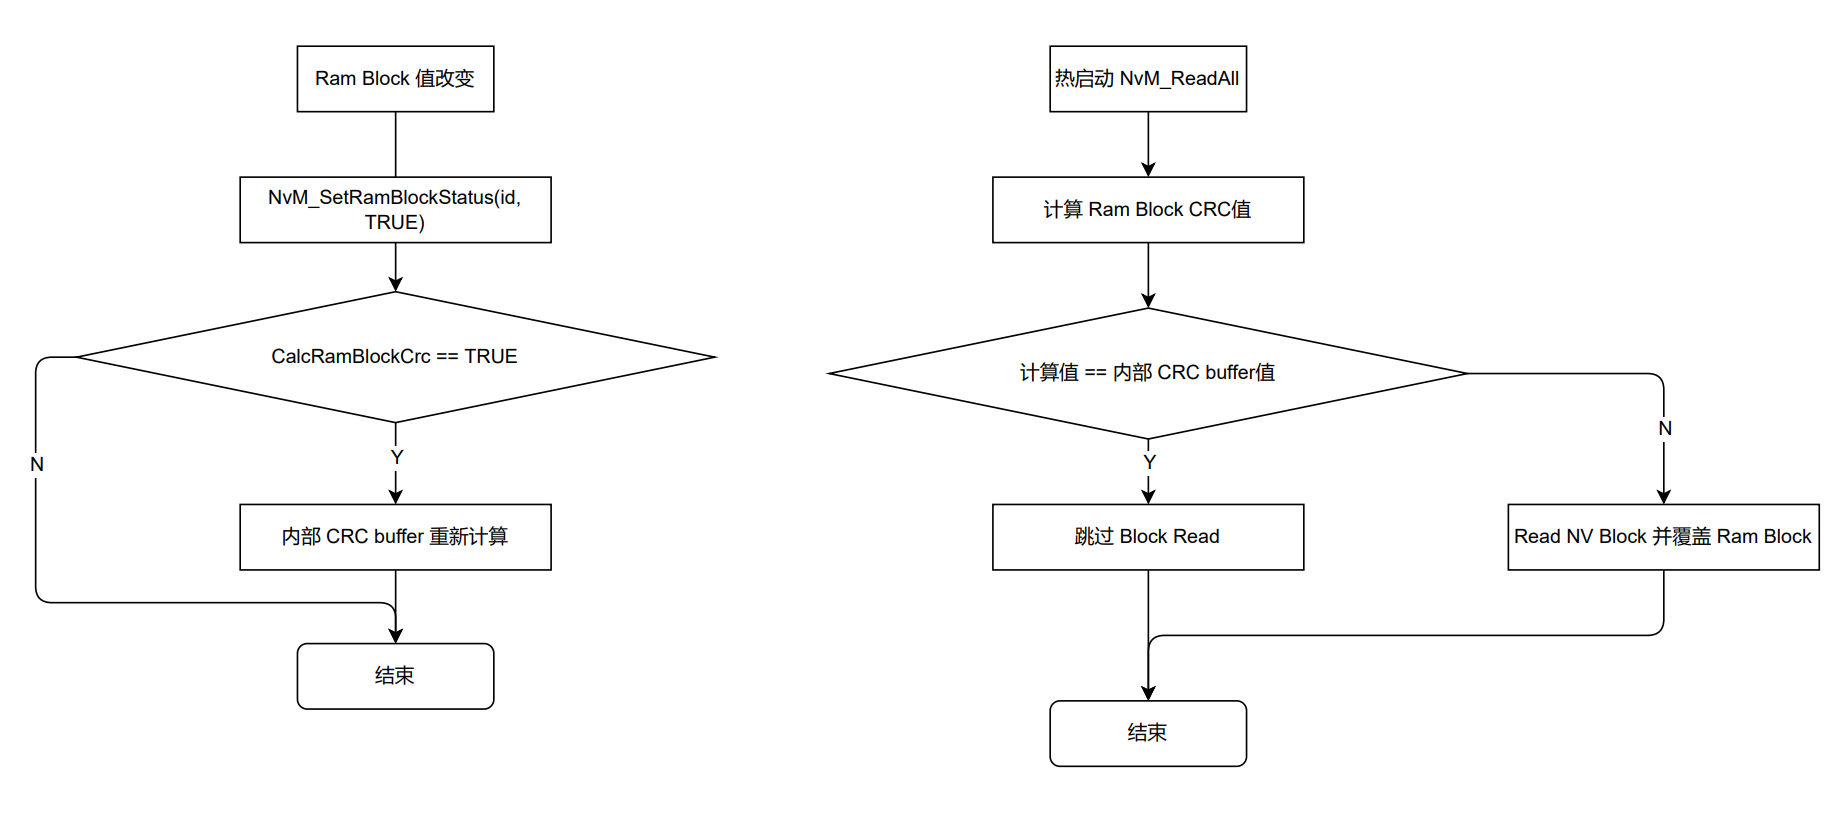
\includegraphics[scale=0.35]{pic/NVM_cal_ram_crc.png}
  \caption{NvMCalcRamBlockCrc 处理流程}
  \label{fig:NVM_cal_ram_crc}
\end{figure}

对于某些 NVRAM 块,可能需要在 \lstinline{NvM_ReadAll} 期间保护相应 RAM 块的数据内容不被覆盖,以防存储在相应 NV 块中的数据比 RAM 块中的数据更旧。例如以下场景,当 RAM 中的数据尚未写入 NV 存储器时热复位。
在这种情况下,RAM 块必须分配在复位安全(不经历初始化)的 RAM 区域中,并且配置参数 CalcRamBlockCrc 必须设置为 \lstinline{TRUE}。 这意味着相应的 NV 块也具有/具有 CRC 配置,并且参数 \lstinline{NvMSetRamBlockStatus} Api 必须设置为值 \lstinline{TRUE} 。

每次更改 RAM 块数据内容后,必须为相应的 NVRAM 块调用 API \lstinline{NvMSetRamBlockStatus} ,并将参数 \lstinline{BlockChanged} 设置为 \lstinline{TRUE} 。然后,NVM 将重新计算此 RAM 块的 CRC,并将结果存储在分配在复位安全(不经历初始化)RAM 区域中的内部变量中。
作为此 NVRAM 块的先决条件,必须配置有效的永久 RAM 块 (NvMRamBlockDataAddress) 或显式同步回调函数 (NvMReadRamBlockFromNvM)。

在每次启动 (\lstinline{NvM_ReadAll}) 期间,NvM 模块都会计算此类 RAM 块的 CRC,如果它与存储的 CRC 值匹配,则不会覆盖 RAM 块。如果计算出的 CRC 与存储的 CRC 不匹配,RAM 块将被从 NV 块读取的数据覆盖,或者,如果此读取尝试失败,
使用默认数据恢复(如果通过参数 NvMRomBlockDataAddress 或参数 NvMInitBlockCallback 配置)。

\subsubsection{NvMBlockUseCrc}
block是否使用CRC。


\subsubsection{NvMBlockUseCRCCompMechanism}

block是否使用compare mechanism。

如果特定ram block对应的NV data在运行时没有更新,为了避免不必要的 NV 写操作,提供了compare
mechanism机制。即,在向NV写数据之前,重新计算当前ram数据的CRC值,并和之前读或写数据操作时保存的CRC值进行比较。

\subsubsection{NvMCrcIntBuffer}

NVM是否内部分配buffer用于CRC校验处理,如果不开启,则每个ram block需要应用程序为各 block 提供空间存储CRC。
当开启内部buffer后,用户数据被拷贝至buffer,然后附加上CRC信息,最后一起被送至下层模块处理。

% \subsubsection{异步 CRC 计算}
% Block 的CRC 值总是在 \lstinline{NvM_MainFunction}中异步计算。
% 当要写入一个Block 到NV 中,则Block 块的 CRC 值总要提前计算。如果读取一个 block,则读取数据的 CRC 值会重新计算并和 NV 中存储的 CRC 值和存储在其他地方的值进行比较。
% 如果一个 Block 勾选了配置 NvMCalcRamBlockCrc ,则其最近计算的 CRC 值将存储在 RAM 中供以后使用。在此配置下,如果一个 block 调用了
% \lstinline{NvM_SetRamBlockStatus(TRUE)}, 则 Ram block 的CRC 值将重新计算。

\subsubsection{异步CRC校验}

block对应的CRC校验是在\lstinline{NvM_MainFunction}中异步进行的。受CRC保护的block在写数据到NV前,都需要计算CRC值。如果从NV中读取数据,CRC的值需要重新计算并和读取到的CRC值进行比较。如果配置了\lstinline{NvMCalcRamBlockCrc},最近计算到的CRC值将存储在RAM中,便于后续使用。

如果调用了
\lstinline{NvM_SetRamBlockStatus(TRUE)},且为此块启用了\lstinline{NvMCalcRamBlockCrc},则还将启动对RAM块数据的CRC值的重新计算。

NvM 在 \lstinline{NvM_ReadAll} 处理期间尝试对所有在其配置中启用了 \lstinline{Read during ReadAll} 和 \lstinline{Calc RAM CRC} 的
NVRAM 块进行尝试:如果块在内部仍标记为 VALID,NVM 将计算当前 RAM
块内容的 CRC 值和存储在其他地方的值进行比较。 如果它们匹配,则不会触及
RAM 内容; 相反,NVM 假装已成功从 NV 读取这些值。

\begin{itemize}
\item
  如果匹配,则无需写操作,并成功结束任务。
\item
  如果不匹配,则需要向NV中写数据。
\end{itemize}

CRC Compare Mechanism和 NvMCalcRamBlockCrc
没有依赖关系,这两者各自使用独立的CRC buffer。

\begin{itemize}
\item
  NvMCalcRamBlockCrc:
  调用 \lstinline{NvM_SetRamBlockStatus} 将引起CRC值的重新计算,NVM保存当前ram
  block数据的CRC值,并在read all时避免真实的从NV
  中读取数据。详见 异步CRC校验。
\item
  Compare Mechanism:
  NVM保存上一次成功读取或写入数据对应的CRC值,如果该CRC值与ram
  block的数据CRC值匹配,则调用\lstinline{NvM_WriteBlock, NvM_WriteAll}时可避免不必要的数据写入。
\end{itemize}

\subsection{API 分析}
\subsubsection{\lstinline{NvM_QueuePop}}

从 Queue 中 pop 第一个job, job 的索引值作为参数返回,入口参数为指针,同样,原 Queue 将指向 pop 元素的下一个元素。

\begin{lstlisting}[language=C,style=C]
  /**********************************
  * NvM_QueuePop
  ***********************************/
 /*! \brief Removes first element from queue.
  *  \details Pops the first element from the given list, i.e. the element is removed from the list and will be returned.
  *           The given list shall not be empty!
  *  \param[in,out] Queue as an index to the queue to pop out of the queue. Caller has to ensure validity.
  *  \return given element's index
  *  \context TASK
  *  \reentrant FALSE
  *  \synchronous TRUE
  *  \config Configuration class is > 1
  *  \pre -
  */
NVM_LOCAL FUNC(NvM_QueueEntryRefType, NVM_PRIVATE_CODE) NvM_QueuePop(NvM_QueueListHeadRefType Queue);
\end{lstlisting}

\subsubsection{\lstinline{NvM_QueuePush}}
在 Queue 中 push 一个元素,队列的第一个元素变为刚入栈的元素。

\begin{lstlisting}[language=C,style=C]
  /**********************************
  * NvM_QueuePush
  ***********************************/
 /*! \brief Add job to queue.
  *  \details Pushes the given element onto the given list, i.e. the element is inserted at list head.
  *  \param[in] Queue as an index to the next queue element. Caller has to ensure validity.
  *  \param[in] Elem as an index to the queue, shall be enqueued at the end of the linked list.
  *             Caller has to ensure validity.
  *  \context TASK
  *  \reentrant FALSE
  *  \synchronous TRUE
  *  \config Configuration class is > 1
  *  \pre -
  */
 NVM_LOCAL FUNC(void, NVM_PRIVATE_CODE) NvM_QueuePush(NvM_QueueListHeadRefType Queue, NvM_QueueEntryRefType Elem);
\end{lstlisting}

\subsubsection{\lstinline{NvM_ActGetNormalPrioJob}}
取出 有效 job queue,即 \lstinline{NvM_NormalPrioQueue.SrvList} 中最先入栈的 job ,并将该 job 的信息保存到 \lstinline{NvM_CurrentJob_t}中。
之后有效队列继续指向最先入队的 job。空队列则入栈一个 job 空位。

\begin{lstlisting}[language=C,style=C]
  /**********************************
  * NvM_ActGetNormalPrioJob
  ***********************************/
 /*! \brief Setups the NvM internal job variable for next job.
  *  \details Scans the given queue for the entry with highest priority, located nearest to the list end.
  *           The element is removed from the list, but stored in NvM_lastJobEntry. The job parameters will be copied
  *           to the passed job structure. The queue is expected to contain at least one element.
  *  \context TASK
  *  \reentrant FALSE
  *  \synchronous TRUE
  *  \config Configuration class is > 1
  *  \pre -
  */
  FUNC(void, NVM_PRIVATE_CODE) NvM_ActGetNormalPrioJob(void)
  {
      NvM_QueueEntryRefType elem;
  
      NvM_EnterCriticalSection();
      /* just take the last queue element, don't store it in NvM_LastJobEntry (it does not exist),
       * but remove it from the queue.
       * Just update the queue head to point to its prev element (which is the tail), then pop.
         After that, the head points to the head again.
       */
      NvM_NormalPrioQueue.SrvList = NvM_JobQueue_at[NvM_NormalPrioQueue.SrvList].PrevEntry;
      elem = NvM_QueuePop(&NvM_NormalPrioQueue.SrvList); /* SBSW_NvM_FuncCall_PtrParam_Queue */
  
      /* free the element --> add it to free-list */
      NvM_QueuePush(&NvM_NormalPrioQueue.EmptyList, elem); /* SBSW_NvM_FuncCall_PtrParam_Queue */
  
      NvM_CurrentJob_t.JobBlockId_t = NvM_JobQueue_at[elem].BlockId;
      NvM_CurrentJob_t.JobServiceId_t = NvM_JobQueue_at[elem].ServiceId;
      NvM_CurrentJob_t.RamAddr_t = NvM_JobQueue_at[elem].RamAddr_t;
  
  
      NvM_ExitCriticalSection();
  }
\end{lstlisting}